\documentclass[conference]{IEEEtran}
\IEEEoverridecommandlockouts
% The preceding line is only needed to identify funding in the first footnote. If that is unneeded, please comment it out.
\usepackage{cite}
\usepackage{amsmath,amssymb,amsfonts}
\usepackage{algorithmic}
\usepackage{graphicx}
\usepackage{textcomp}
\usepackage{xcolor}
\def\BibTeX{{\rm B\kern-.05em{\sc i\kern-.025em b}\kern-.08em
    T\kern-.1667em\lower.7ex\hbox{E}\kern-.125emX}}
\begin{document}

\title{Image Super-Resolution}

\author{

\IEEEauthorblockN{Giuseppe Di Blasi}
\IEEEauthorblockA{
\textit{University of Parma}\\
giuseppe.diblasi@studenti.unipr.it}

}
\maketitle

\begin{abstract}
La super-resolution è una tecnica di computer vision che mira a ricostruire immagini ad alta
risoluzione a partire da immagini a bassa risoluzione.
In questo progetto sono state implementate e valutate diverse
architetture di reti neurali convoluzionali ispirate ai modelli SRCNN e VDSR.
I modelli sono stati addestrati sul dataset DIV2K e valutati sul benchmark Set5
utilizzando il PSNR come metrica principale. Sono state inoltre analizzate diverse
modifiche architetturali, tra cui l'aumento della profondità della rete, il residual learning,
la batch normalization e l'utilizzo di differenti funzioni di loss. I risultati ottenuti mostrano
che la loss L1 ha fornito le migliori prestazioni, consentendo in alcuni casi di superare
l'interpolazione bicubica e di ottenere un miglioramento percettivo della qualità delle immagini
ricostruite.
\end{abstract}


\section{Introduzione}
Il progetto è incentrato sulla Super Resolution,
ovvero una tecnica per migliorare la risoluzione
di immagini a bassa qualità.

Vengono mostrati diversi approcci come le reti CNN e le reti residuali.
Il dataset utilizzato per la fase di test e di validazione è stato preso da DIV2K.
Per il dataset di test è stato utilizzato Set5.

Il progetto ha preso in considerazione lavori già pubblicati in precedenza nel
contesto della super resolution, cercando di ottenere
gli stessi risultati anche con approcci diversi.


\section{Architettura CNN}

\subsection{Fonti accademiche, dataset e metriche di valutazione}
Come primo approccio al problema della super-resolution è stata implementata
 una rete neurale convoluzionale
 (CNN) basata sul modello SRCNN \cite{dong2014srcnn}, che ha mostrato prestazioni superiori rispetto ai metodi di interpolazione tradizionali, come l'interpolazione bicubica.

Per l'addestramento e la validazione è stato utilizzato il dataset DIV2K,
composto da 800 immagini ad alta risoluzione (2K).
La fase di test è stata invece eseguita sul dataset Set5,
comunemente utilizzato come benchmark per la valutazione di algoritmi di super-resolution.

Inizialmente le prestazioni del modello sono state valutate tramite il valore della loss.
 Successivamente è stato adottato il PSNR (\textit{Peak Signal-to-Noise Ratio}),
  calcolato confrontando le immagini ricostruite con le corrispondenti ground truth.
  Tale metrica è stata utilizzata sia per valutare il modello sia per confrontarne
  le prestazioni con quelle ottenute mediante interpolazione bicubica.

Come funzione di perdita è stata inizialmente
utilizzata la MSE (\textit{Mean Squared Error}), seguendo la scelta del paper SRCNN\cite{dong2014srcnn}.
 In una seconda fase sono stati condotti esperimenti utilizzando la
 L1 loss (\textit{Mean Absolute Error})
  per valutarne l'impatto sul processo di addestramento e sulle prestazioni finali.

\subsection{Pre-upsampling immagini}

In accordo con l'approccio SRCNN,
l'operazione di upsampling non viene eseguita dalla rete
 ma tramite interpolazione bicubica prima dell'inferenza.
 La CNN riceve quindi in ingresso un'immagine già riportata
 alla risoluzione target e apprende a migliorarne la qualità,
 recuperando dettagli e riducendo gli artefatti introdotti dall'interpolazione.

\begin{figure}[ht]
    \centering

    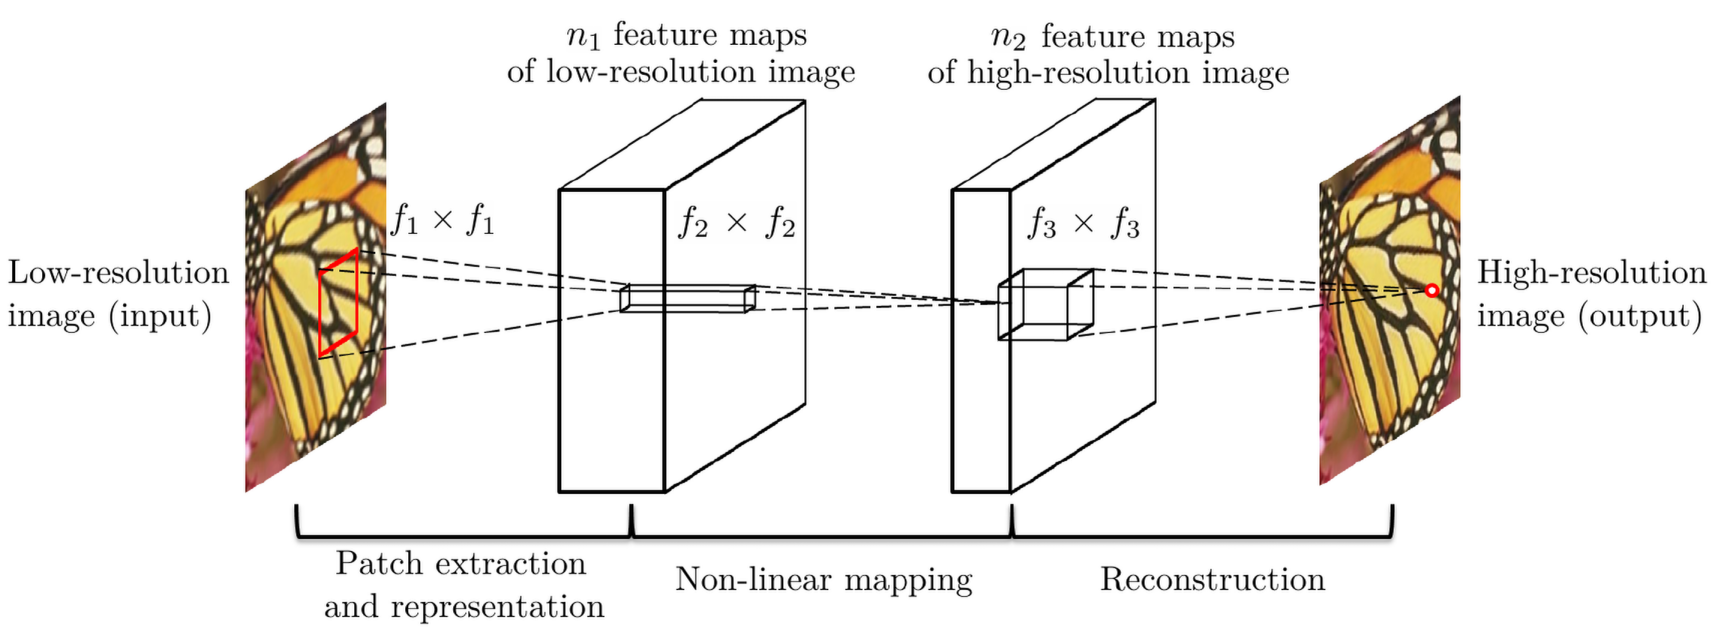
\includegraphics[width=0.8\columnwidth]{figures/architettura_SRCNN.png}
    \caption{Architettura della rete CNN, primo layer è per la feature extraction;
    il secondo per non-linear mapping
    e il terzo cerca di abbinare le predizioni della rete all'immagine ad alta risoluzione}

    \vspace{0.5cm}

    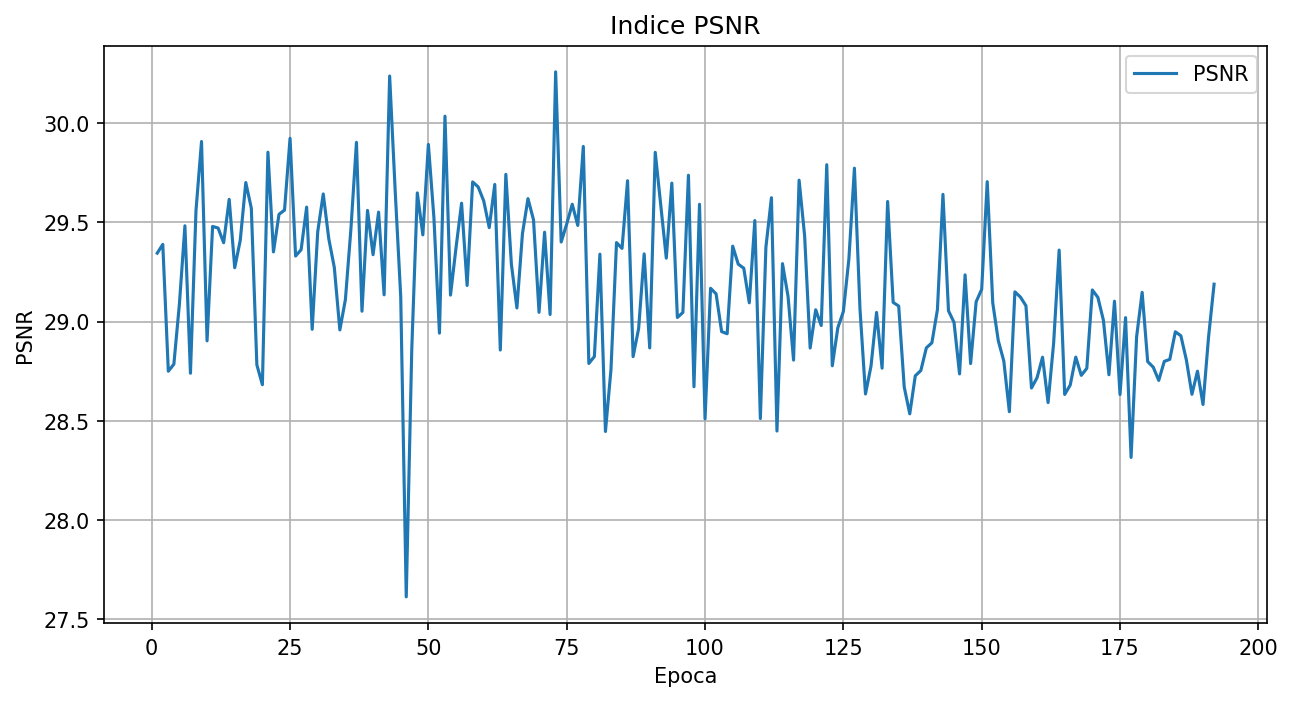
\includegraphics[width=0.8\columnwidth]{figures/srcnn_600_9-5-5-5-5-5-5_BN_L1_psnr_plot.png}
    \caption{Kernel: 5x5, BN, L1 Loss}

\end{figure}
\section{Risultati con rete SRCNN\cite{dong2014srcnn}}

La fase di training è stata strutturata nel seguente modo:
800 immagini da cui vengono estratte casualmente 20 patch, di grandezza 64x64,
per ogni immagine, ottenendo così circa 16.000 patch per la fase di addestramento.
A differenza del paper SRCNN\cite{dong2014srcnn}
abbiamo scelto di provare a passare i 3 canali RGB come input alla rete invece del canale
di luminanza, ottenendo dei risultati per niente soddisfacenti,
la rete generava un output che presentava parecchi artefatti.

\begin{figure}[ht]
    \centering
    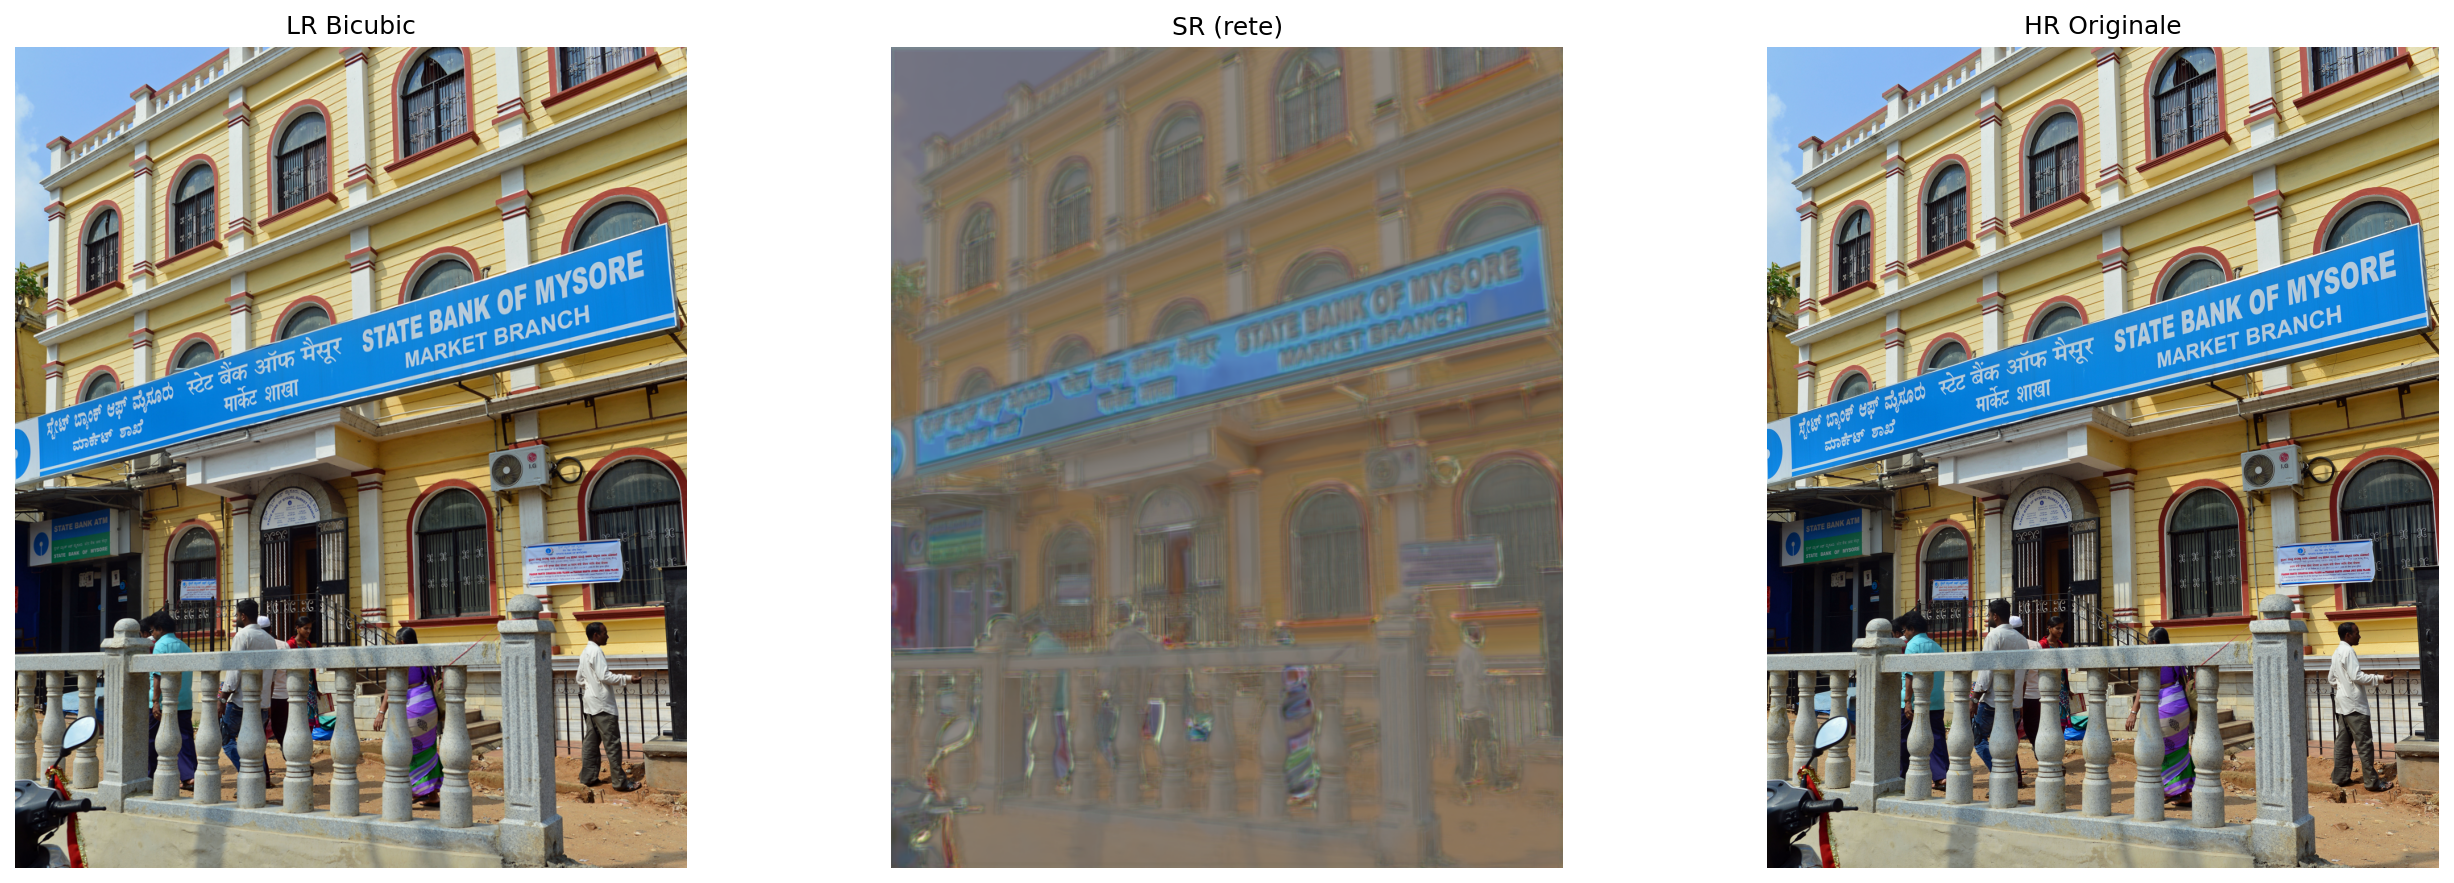
\includegraphics[width=\columnwidth]{figures/confronto_srcnn_150_epochs_2026-05-20_11-07-06.png}
    \caption{Output rete con RGB come input.}
    \label{fig:sr_artefatti_rgb}
\end{figure}

Dopo gli scarsi risultati ottenuti si è deciso di passare solo il canale della luminanza
(Y) alla rete, seguendo quello che è stato fatto nel paper SRCNN\cite{dong2014srcnn}.

Andando a riprodurre l'architettura con 3 layer,
con kernel di grandezza, rispettivamente 9x9, 5x5, 5x5;
con 64 canali in output dal primo layer, con un learning rate di $10^{-4}$ per i
primi 2 layer e per l'ultimo $10^{-5}$.
Abbiamo ottenuto dei risultati migliori rispetto all'approccio RGB,
ma non riuscivamo a superare il PSNR dell'algoritmo di interpolazione Bicubic.

\begin{figure}[ht]
    \centering
    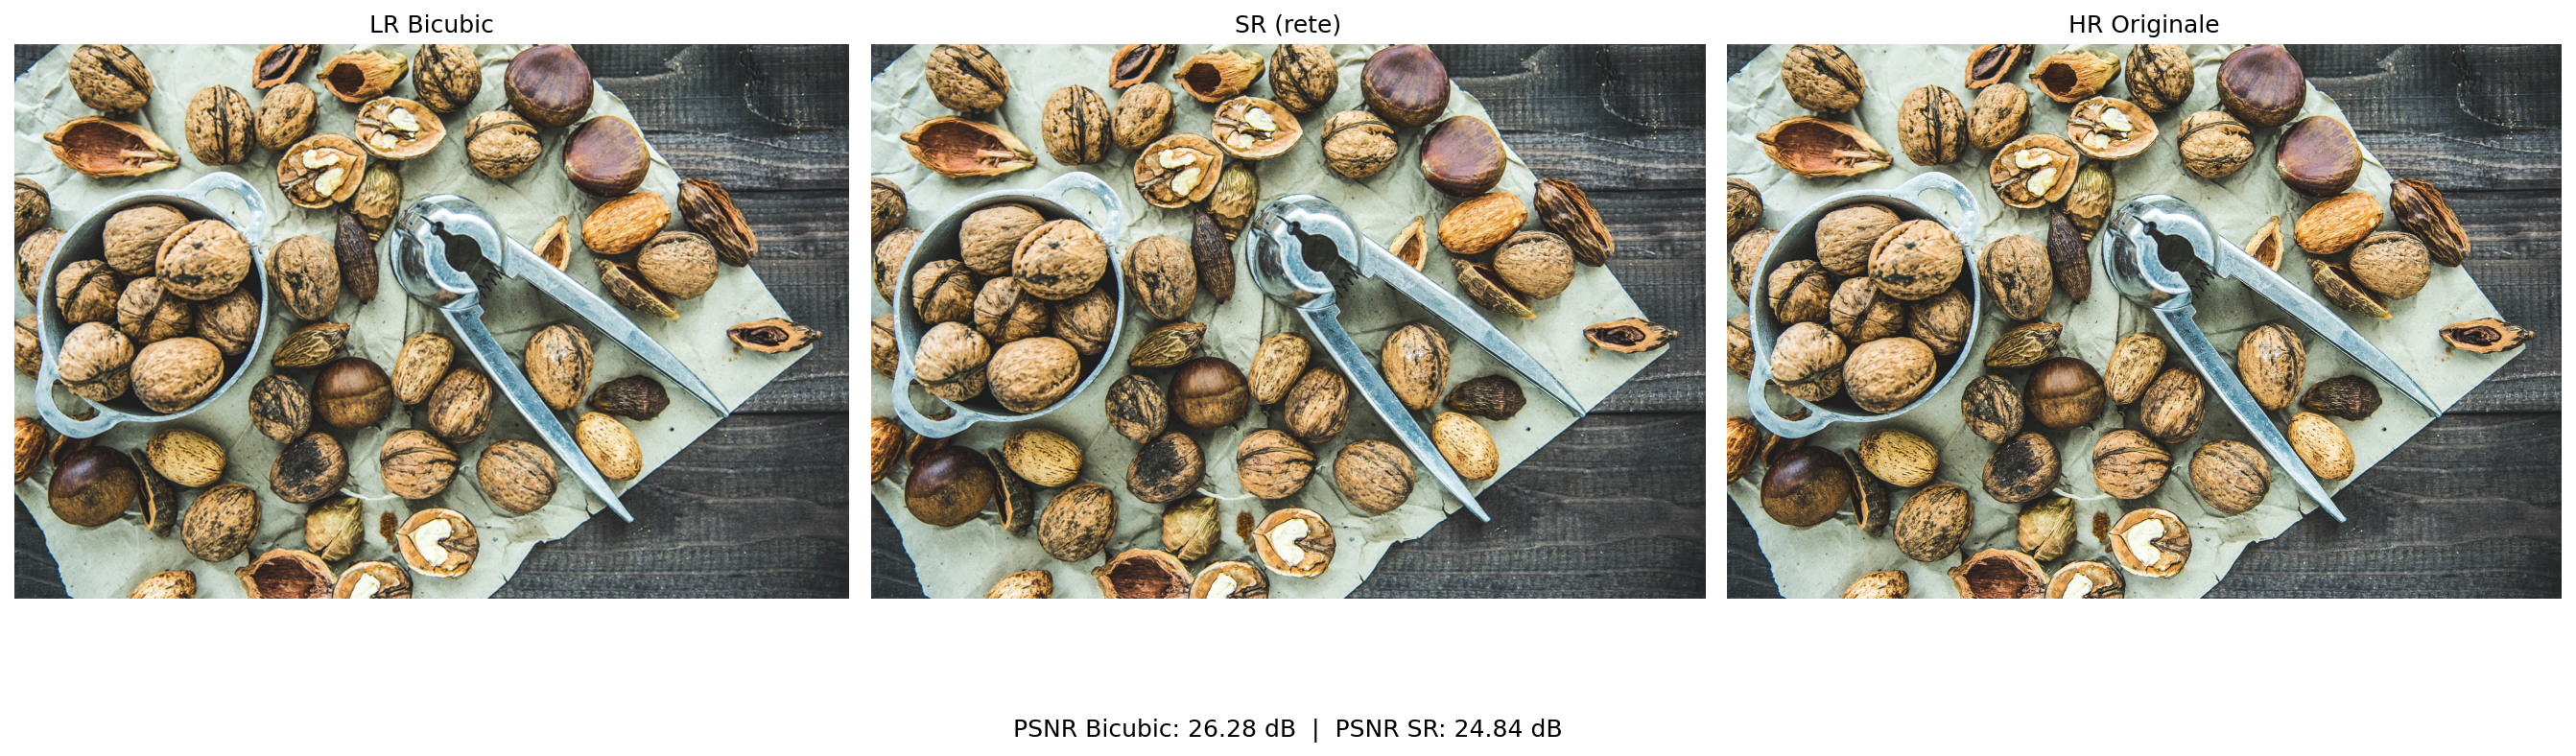
\includegraphics[width=\columnwidth]{figures/confronto_srcnn(9-5-5)_model_600_epochs_2026-05-23_13-06-36.png}
    \caption{Output della rete con input luminanza (Y).
PSNR Bicubic: 26.28 dB, PSNR SR: 24.84 dB}
    \label{fig:sr_Y}
\end{figure}

La fase di validazione è stata fatta estraendo una patch centrale delle
stesse dimensioni delle patch usate per il training, sfruttando il dataset di validation di DIV2K.
In questo modo siamo stati in grado di stabilire come le prestazioni
reali della rete si evolvessero durante la fase di training.

Per la fase di test la rete lavora sull'immagine intera invece delle patch.

Con l'architettura del paper non siamo riusciti a superare bicubic in nessuna istanza del test set,
forse dovuto anche al fatto che abbiamo utilizzato un dataset di training diverso.
\section{Esperimenti sull’architettura e sulla funzione di loss}

Non soddisfatti dei risultati abbiamo cambiato l'architettura della rete,
passando a 7 layer di convoluzione, lavorando sempre sul canale Y.

\subsection{Modifiche per fase di training}

Il numero di patch estratte per immagine durante il training è stato aumentato da 20 a 40,
ottenute dal dataset DIV2K di 800 immagini, portando il numero totale di campioni a circa 32 mila.
La grandezza delle patch è stata aumentata da 64 a 128,
in modo di permettere alla rete di vedere più informazioni.

\subsection{Modifiche all'architettura}
Il primo layer di convoluzione ha un kernel di $9\times9$ mentre i
restanti hanno kernel con grandezza $3\times3$.
Come loss function abbiamo mantenuto la MSE tra l'immagine di output
dalla rete e la ground truth, ovvero l'immagine ad alta risoluzione.
Il learning rate è stato fissato a $10^{-4}$ per tutti i layer stavolta.

Aumentando il numero di layer ci aspettiamo di
ottenere potenziali miglioramenti per quanto riguarda l'output della rete.

Abbiamo inserito anche un early stopping per evitare di sprecare tempo durante la fase di training, se la rete non migliora il proprio PSNR globale per 120 epoche consecutive il training si ferma.

Con questa nuova architettura ci siamo avvicinati ai valori PSNR dell'algoritmo bicubic ma ancora non abbastanza da poter superarlo.

È stato inoltre valutato il residual learning.
In questo approccio, la rete non apprende direttamente la mappatura dall’immagine a bassa risoluzione (LR) a quella ad alta risoluzione (HR),
ma la differenza residua tra le due.
In questo modo il modello non modifica la struttura dell’architettura in senso ResNet,
ma cambia semplicemente la quantità che la rete è chiamata a stimare.

Questi cambiamenti sono stati presi dal paper VDSR \cite{kim2015accurate}.

\begin{figure}[ht]
    \centering

    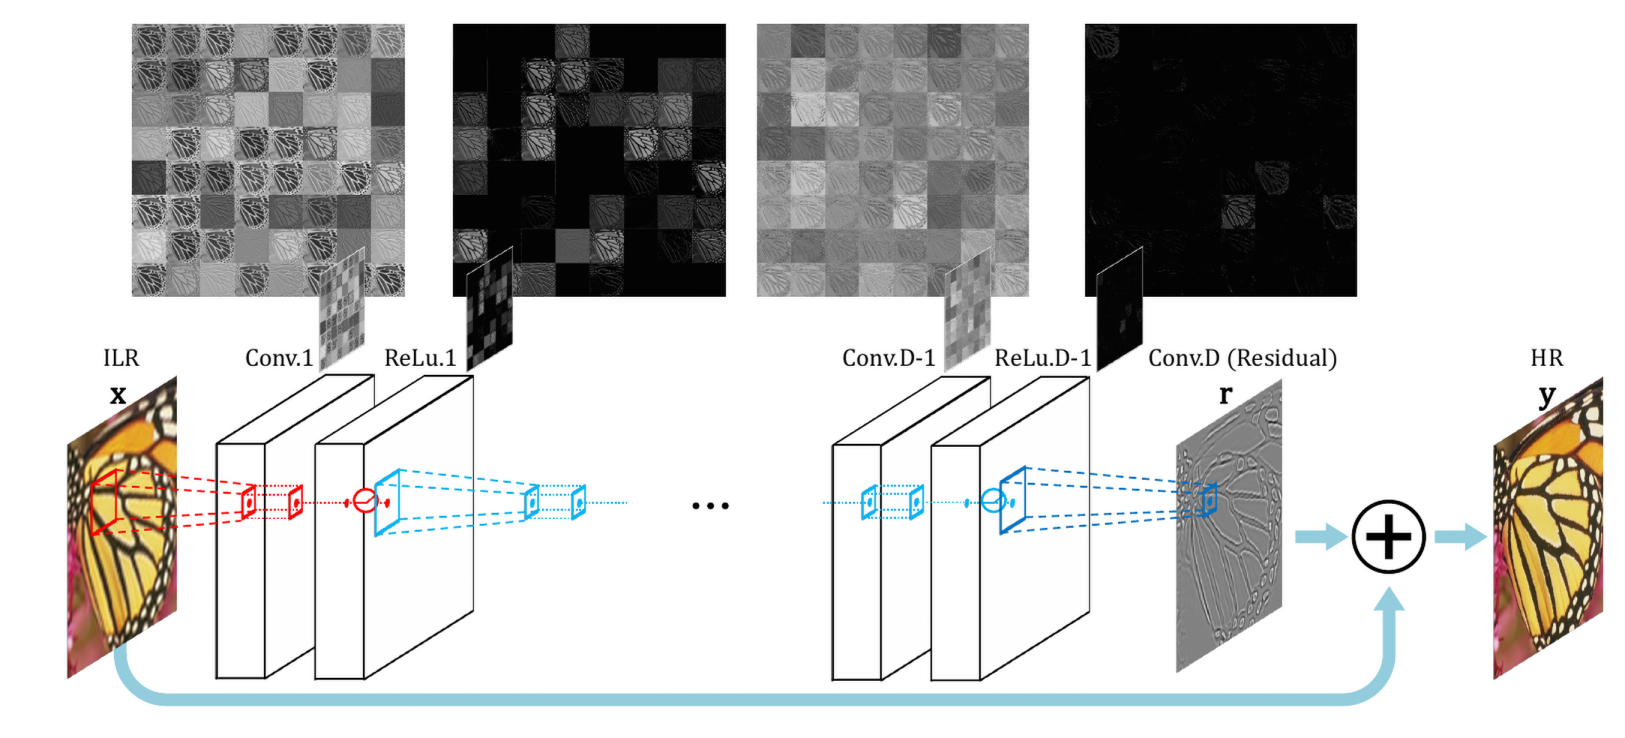
\includegraphics[width=1\columnwidth]{figures/architettura_VDSR.png}
    \caption{Architettura rete VDSR}

\end{figure}

\subsection{Differenze con paper VDSR \cite{kim2015accurate}}

Una differenza sostanziale rispetto al modello VDSR \cite{kim2015accurate} riguarda la profondità della rete:
quest’ultimo utilizza 20 layer convoluzionali, mentre nel nostro caso ne sono stati impiegati 7,
al fine di ottenere risultati soddisfacenti in tempi di addestramento più contenuti.

Con questa architettura sono stati ottenuti risultati migliori rispetto al modello SRCNN \cite{dong2014srcnn}.
Tuttavia, in nessuna istanza del test set si è riusciti a superare le prestazioni dell’interpolazione bicubica.

Con questa architettura è stata osservata una variazione instabile del PSNR durante la fase di training.
Per ridurre tale instabilità è stata introdotta la batch normalization dopo ogni layer convoluzionale,
al fine di normalizzare le attivazioni intermedie della rete e stabilizzare il processo di ottimizzazione.

L’introduzione della batch normalization ha portato a una riduzione
delle oscillazioni
del PSNR durante il training; anche questa scelta si discosta da VDSR\cite{kim2015accurate}.

Abbiamo inoltre cambiato la grandezza dei kernel dal
layer 2 al layer 7 da $3\times3$ a $5\times5$, in modo da osservare eventuali
miglioramenti nei risultati, anche se questo si discosta dal paper VDSR \cite{kim2015accurate}
che usava $3\times3$ come grandezza per i kernel dei layer intermedi.


Come ultimo tentativo abbiamo provato a sostituire MSE come funzione di loss con L1.
La MSE eleva al quadrato la differenza penalizzando di
più errori grandi rispetto a quelli piccoli, L1 invece prende il valore assoluto,
dando lo stesso peso a tutti gli errori commessi dalla rete.

\subsection{Risultati finali}

\begin{figure}[ht]
    \centering

    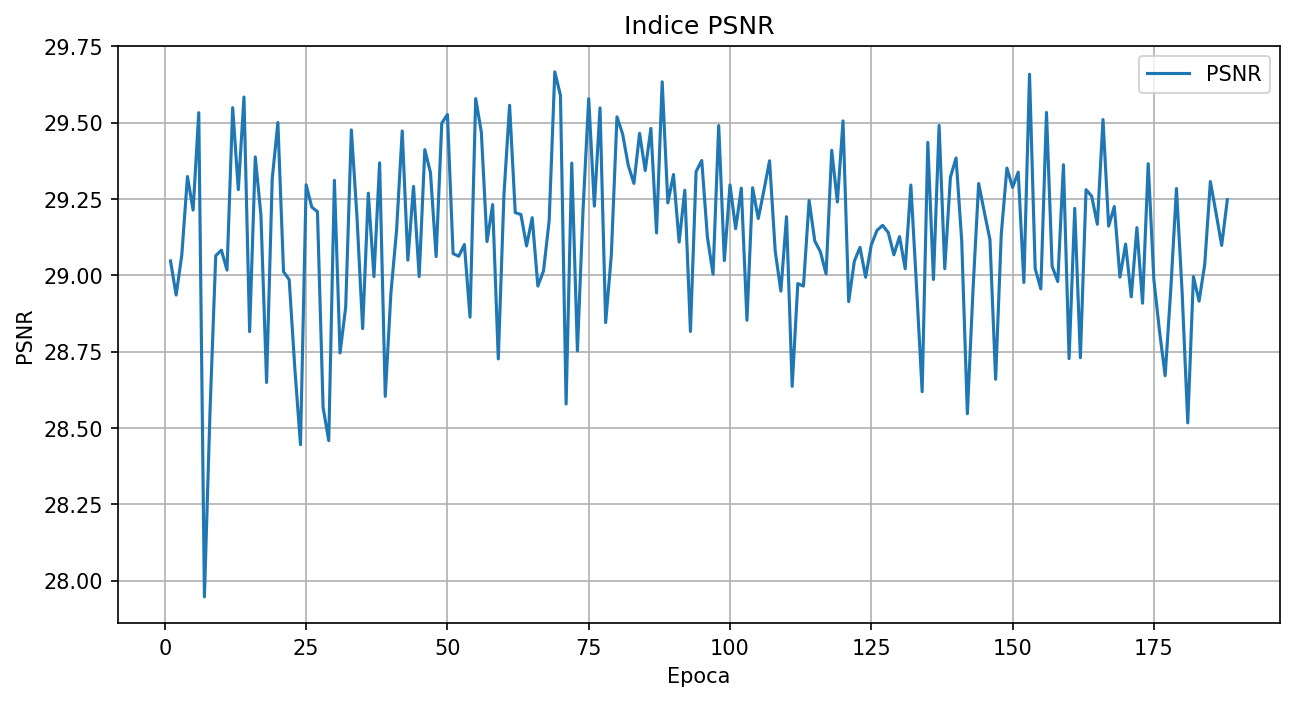
\includegraphics[width=0.8\columnwidth]{figures/srcnn_600_9-3-3-3-3-3-3_psnr_plot.png}
    \caption{Kernel: 3x3; no BN, MSE Loss}

    \vspace{0.5cm}

    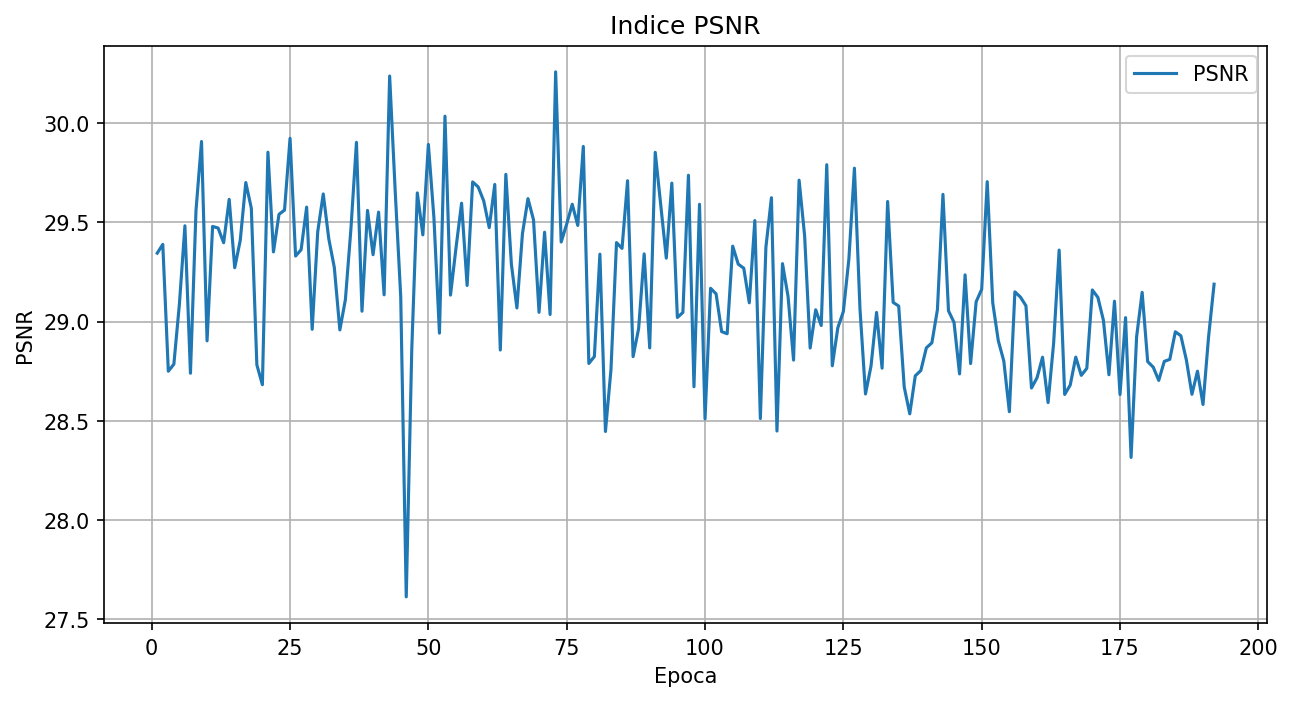
\includegraphics[width=0.8\columnwidth]{figures/srcnn_600_9-5-5-5-5-5-5_BN_L1_psnr_plot.png}
    \caption{Kernel: 5x5, BN, L1 Loss}

\end{figure}

Grazie alla loss L1 siamo riusciti a superare l'algoritmo Bicubic in una istanza del test set,
ottenendo anche un miglioramento  sui dettagli dell'immagine visibile ad occhio nudo.

\begin{figure}[ht]
    \centering
    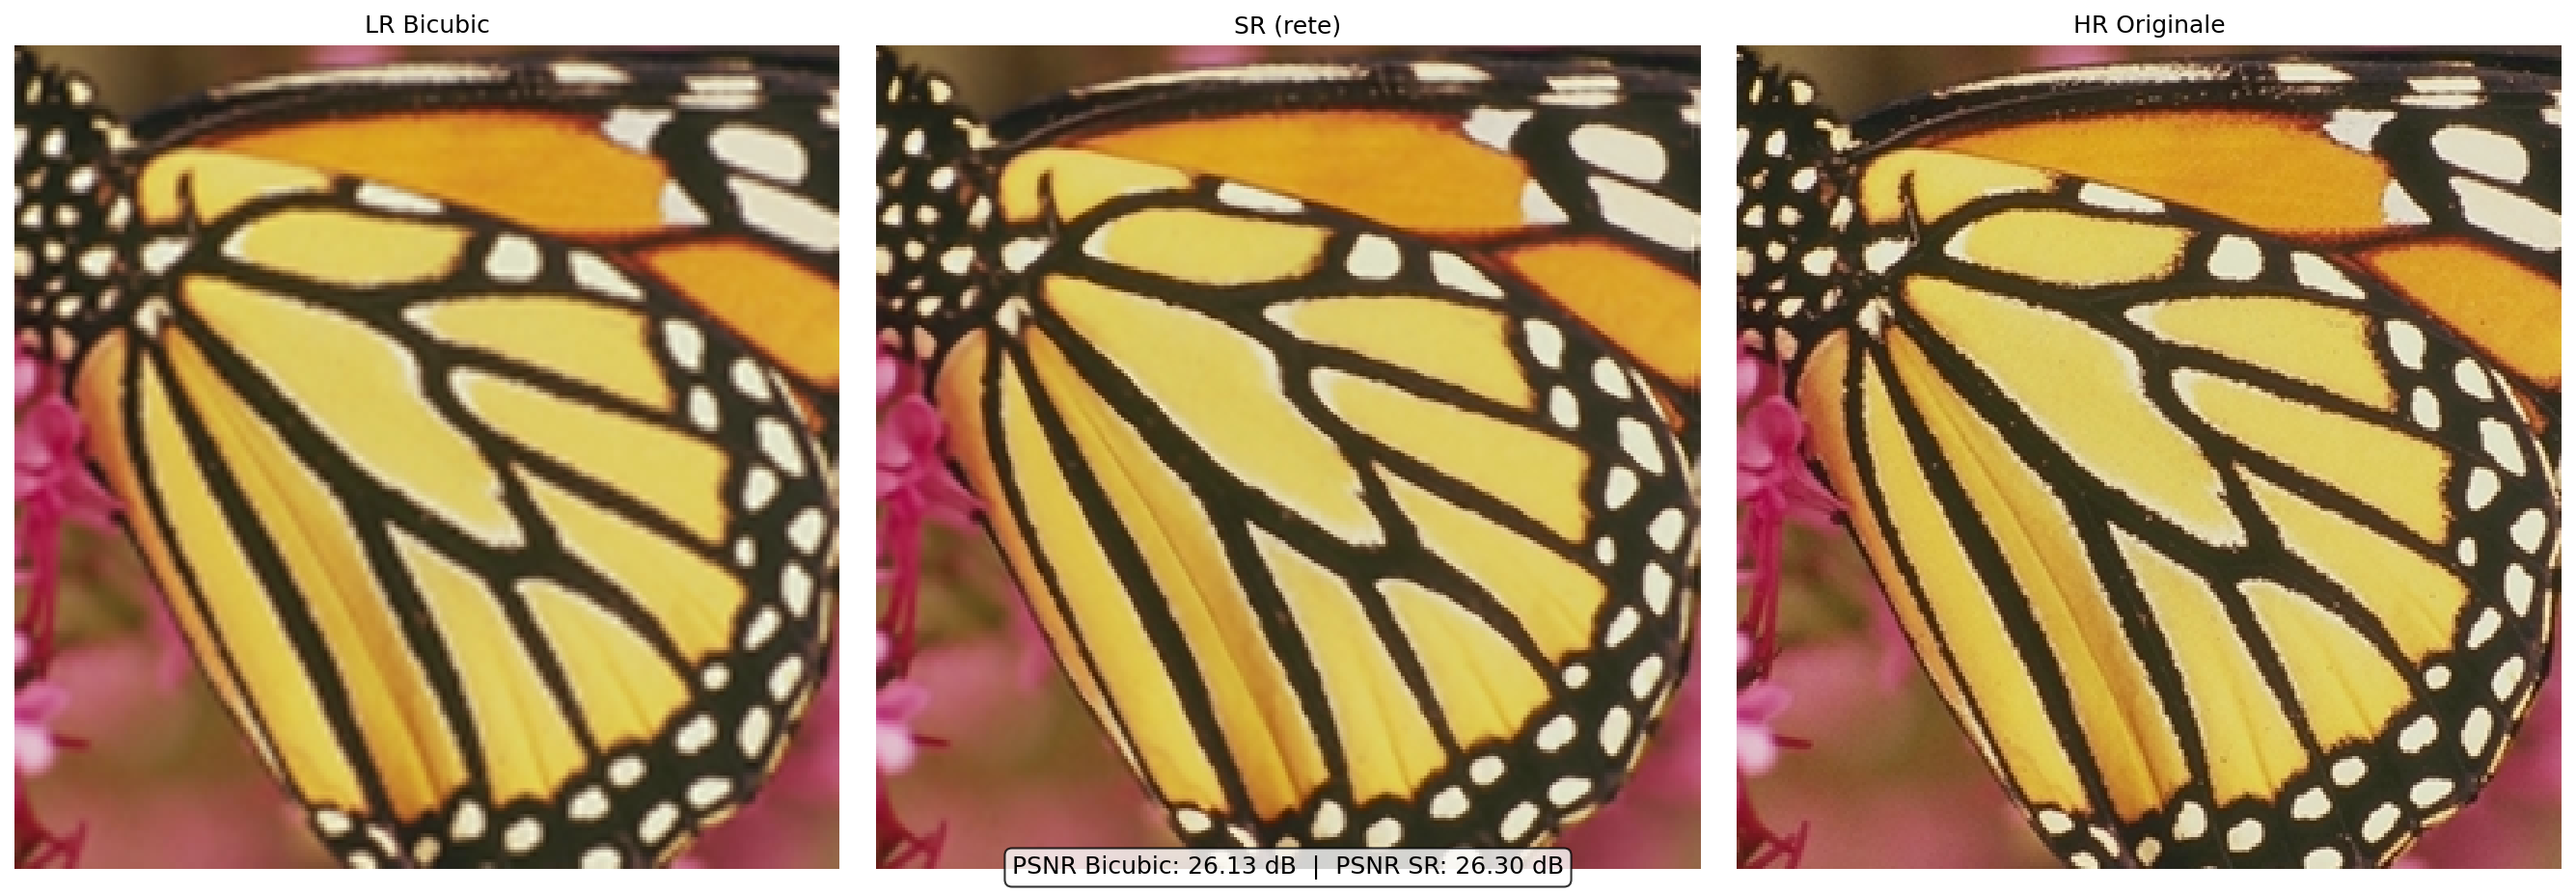
\includegraphics[width=\columnwidth]{figures/risultato_migliore.png}
    \caption{La rete SR supera Bicubic, Bicubic: 26.16 dB, SR: 26.30 dB}
    \label{fig:sr_finale}
\end{figure}

Nonostante l’aumento limitato del PSNR (0.15 dB), si osservano miglioramenti visivi
nelle aree più dettagliate dell’immagine.
Questo evidenzia il limite del PSNR nel rappresentare pienamente la qualità percettiva,
dovuto al fatto che calcoli l'errore pixel per pixel.

\section{Conclusioni}
In questo lavoro sono stati implementati e
confrontati diversi modelli CNN per la super-resolution ispirati
a SRCNN\cite{dong2014srcnn} e VDSR\cite{kim2015accurate}.
 Nonostante i miglioramenti progressivi introdotti,
 le prestazioni non hanno superato sistematicamente l'interpolazione bicubica.
 Il risultato migliore è stato ottenuto con la loss L1,
 che ha permesso di superare Bicubic in un caso del test set con un
 miglioramento percettivo visibile sui dettagli.
 La difficoltà nel raggiungere prestazioni superiori è probabilmente
 attribuibile all'utilizzo di un dataset di training diverso rispetto ai paper di riferimento,
 all'assenza di data augmentation e a una profondità della rete ridotta.
 Il fatto che la loss si stabilizzasse dopo circa cento epoche suggerisce
 inoltre che il modello raggiungeva i limiti della propria capacità rappresentativa,
 indipendentemente dalla durata dell'addestramento.
%\input{sections/03_Prepare_Your_Paper_Before_Styling}
%\section*{Acknowledgment}

The preferred spelling of the word ``acknowledgment'' in America is without 
an ``e'' after the ``g''. Avoid the stilted expression ``one of us (R. B. 
G.) thanks $\ldots$''. Instead, try ``R. B. G. thanks$\ldots$''. Put sponsor 
acknowledgments in the unnumbered footnote on the first page.



\bibliographystyle{IEEEtran}
\bibliography{Riferimenti}
\end{document}
